\documentclass[12pt]{article}
\usepackage{graphicx}
\usepackage{hyperref}
\usepackage{amsmath}
\usepackage{amssymb}
\usepackage{geometry}
\geometry{a4paper, margin=1in}
\usepackage{times}  % Ensures Times New Roman or closest equivalent
\usepackage{setspace}  % For line spacing
\usepackage{ragged2e}  % Ensures justification
\onehalfspacing
\justifying
\title{\textbf{Content Delivery Network}\\ \large Distributed Systems}
\author{Krish Khimasia \and Thoyajakshi Gorantla \and Tanishq Prasad}
\date{\today}

\begin{document}
\maketitle

\begin{abstract}
The Internet is inherently decentralised, which has been a key factor in its rapid growth
and evolution. While this decentralisation has allowed it to scale efficiently, it has also
made it challenging to guarantee consistent performance and systematically address
network inefficiencies. With the growing demand for high-speed web services delivering
various types of multimedia content, which is straining network bandwidth and server
capacity, a Content Distribution Network (CDN) serves as an effective solution to
enhance Internet service quality.

CDNs have emerged as a crucial solution to address these scalability and performance
challenges. By leveraging a network of geographically distributed servers, CDNs cache
and serve content closer to users, reducing latency and alleviating the load on origin
servers. This approach enhances web performance, ensuring faster and more reliable
content delivery. CDNs are widely utilized for various applications, including website
acceleration, multimedia streaming, software distribution, and other bandwidth-intensive
services.

This paper provides an overview of CDNs and examines their key features. It also
discusses the fundamental design considerations and essential design challenges
within a CDN system. Furthermore, we explore CDN architectures and analyze three
practical implementations—Akamai, AWS CloudFront, and Microsoft Azure Front
Door—focusing on their network structures, caching strategies, and performance
optimizations.

Through this analysis, we aim to provide a comprehensive understanding of CDN
technology, its impact on content delivery, and the trade-offs involved in different
implementations.
\end{abstract}

\clearpage
\section*{Preface}
\addcontentsline{toc}{section}{Preface}

The purpose of this report is to study and compare major Content Delivery Networks (CDNs) in use today. Initially, the scope was to explore three prominent CDN solutions. However, due to the limited availability of technical documentation and publicly accessible design papers for some providers we extended our research to cover four.

Among the CDNs reviewed, \textbf{Akamai} stood out as the most extensively documented and well-studied. This allowed us to perform a deeper analysis into its internal workings, particularly focusing on how it delivers different forms of content efficiently. For the other three CDNs, i.e. \textbf{Azure Front Door}, \textbf{Cloudflare}, and \textbf{Amazon CloudFront}, we provide focused overviews, highlighting key architectural choices, feature sets, and distinguishing characteristics that set them apart.

The report is structured to first introduce the general architecture and goals of CDNs. We then examine the specific design patterns, capabilities, and strategic trade-offs made by each CDN provider.


\clearpage
\tableofcontents

\clearpage

\section{Introduction}
The internet is more accessible than ever, with billions of users worldwide connected
through broadband, mobile networks, and satellite technology. All these users are
consuming online content daily at a scale like never before. The decentralized nature of

the internet and the increasing richness of the content consumed make it difficult to
provide performance guarantees. Latency of as short as one second seems to be
annoying for the user today, hence, efforts to mitigate unpredictable performance in
content delivery can provide great incentive.

A Content Delivery Network (CDN) is one such effort that has proved to be effective.
The main concept behind CDN is to make content available to the servers at the edge
of the user network. This is achieved by using a hierarchy of “replica” servers and cache
servers provided by the content provider. The content provider mirrors content in the
“origin” server to the “replica” servers all over the world. When a user requests some
piece of content, the replica server closest to the user serves the request rather than the
origin server, leading to faster response times.

\section{Overview}
\subsection{Features}
\begin{itemize}
    \item \textbf{Caching:} The CDN stores copies of content at multiple servers located closer to the
    users, known as Points of Presence or PoPs.
    \item \textbf{Latency Reduction:} Whenever a client requests a piece of content, the content is
    served by the PoP closest to the client, resulting in faster load times.
    \item \textbf{Load Balancing:} As any piece of content resides in multiple replica servers, the
    requests for it can be redirected and distributed to prevent congestion in any network
    path.
    \item \textbf{Scalability:} Modern CDNs dynamically allocate resources based on demand, ensuring
    optimal performance even under heavy traffic conditions. Dynamic server scaling is
    implemented, allowing CDNs to automatically adjust the number of active servers based
    on real-time traffic demands.
    \item \textbf{Redundancy:} Replication of content over many servers across the globe allows the
    CDN to be redundant, fault tolerant and reliable. In case a particular server is facing a
    lot of traffic or fails, the content on that server will be available on another server to
    which the requests for the failed server can be redirected.
    \item \textbf{Cost optimisations:} A particular CDN can host content provided by multiple content
    providers, allowing one robust infrastructure to be used jointly by them. These providers
    can share costs and enjoy the ability to serve content all around the world reliably at a
    fairly affordable rate. Caching of content also reduces the amount of data to be
    transferred, reducing network bandwidth costs.
    \item \textbf{Security:} CDNs usually provide many security features, such as protection from DDoS
    attacks and encryption of data.
\end{itemize}

\subsection{Design Issues}
There are various details to focus on at every level when it comes to designing a CDN. Every decision involves trade-offs and brainstorming over the use cases that the CDN is primarily designed to handle. Some of these are as follows:
\begin{itemize}
\item \textbf{Pull/Push CDNs}:

\item \textbf{Replica Server Placement}: Deciding where to place the replica servers on the internet is crucial for the performance of the CDN. Intuitively, they should be placed as close to the users as possible. There are theoretical approaches based on the center placement problem to model our problem. This problem is computationally hard, and hence some heuristics have been developed which takes into account existing information of the CDN.

\item \textbf{Object Replica Placement}: This deals with the problem of which servers to place any particular piece of content on. Handling this allows the CDN to balance load and improve performance.

\item \textbf{Request Routing}:

\item \textbf{Distribution System}: The CDNs can distribute content to replica servers using either the internet or broadcast satellite. In internet distribution, the CDN creates and maintains “a distribution tree or overlay network over the existing internet infrastructure” and distributes content from the origin server to the replica servers via this overlay network. This suffers from the unpredictability of the internet itself. Akamai uses this distribution system. Data satellite broadcast appears to be a cost saving alternative that is reliable in providing critical content such as live streams. CyberStar uses this distribution scheme.

\end{itemize}

\section{Architecture}
\subsection{Components}
\begin{itemize}
    \item Client
    \item Origin Servers
    \item Replica servers
    \item Distribution system
    \item Request routing system
    \item Accounting system
    \item Billing organisation
\end{itemize}

\subsection{Distribution and Routing}
\begin{figure}[h]
    \centering
    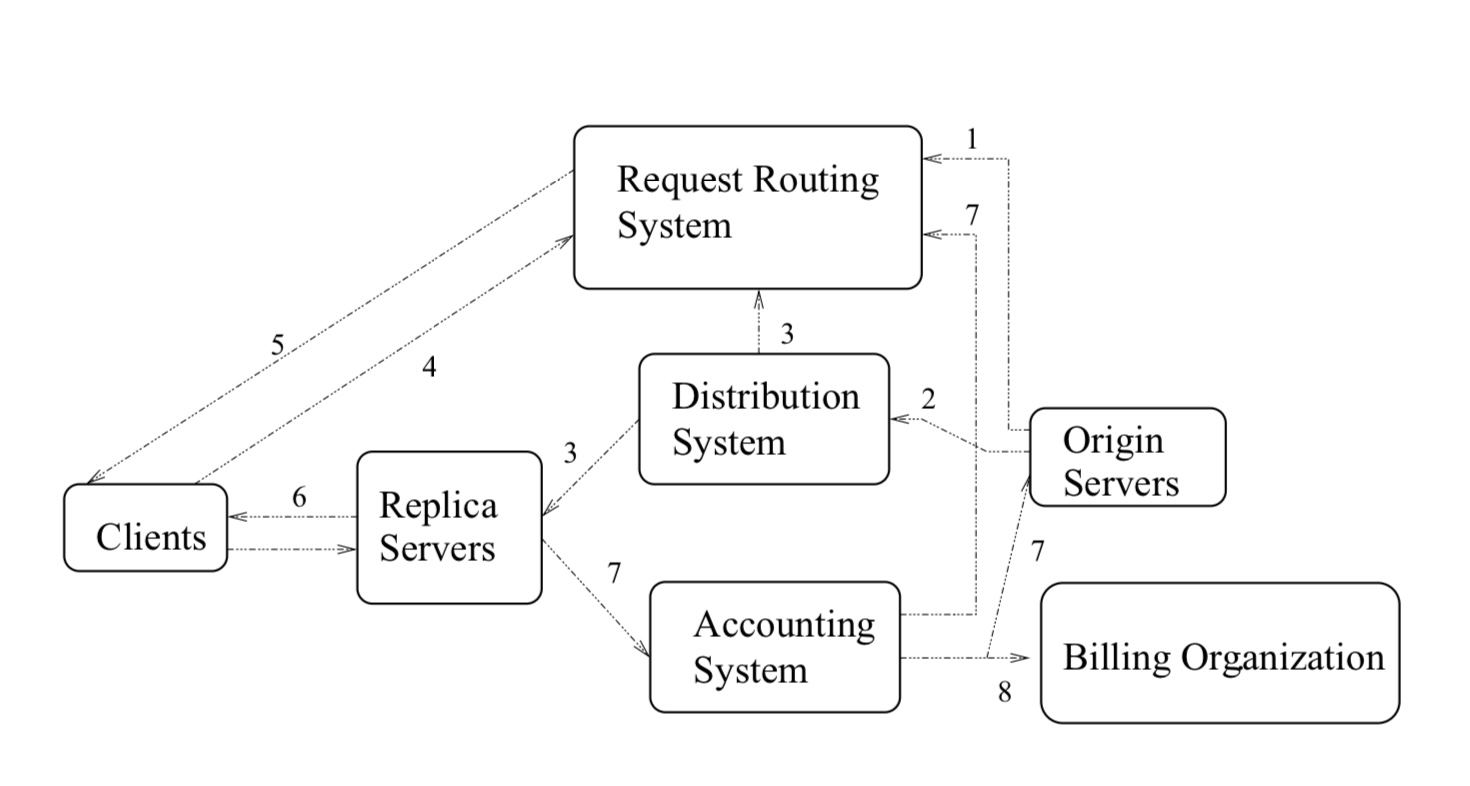
\includegraphics[width=0.8\textwidth]{./imgs/IMG_0281.jpg} % Change filename accordingly
    \caption{An example image showing CDN architecture.}
    \label{fig:cdn_architecture}
    \vspace{0.2cm}
    \small Source: \text{CDN by Gang Peng} % Use actual reference or URL
\end{figure}


\begin{enumerate}
    \item The origin server assigns its URI namespace for document objects to the request routing system, enabling their distribution and delivery by the CDN.
    \item The origin server gives the content that is to be distributed by the CDN to the distribution system.
    \item The distribution system transfers the content to replica servers and works with the request routing system to help determine the appropriate replica server for a client request.
    \item The client initiates requests for documents from what it assumes to be the origin server. However, due to URI namespace delegation, the request is redirected to the request routing system.
    \item The request routing system directs the client request to an appropriate replica server within the CDN.
    \item The corresponding replica server delivers the requested content to the client. Furthermore, the replica server provides the accounting system with data on the content it has delivered.
    \item The accounting system compiles and refines accounting data into statistics and content detail records, which are utilized by the origin server and billing organization. Additionally, these statistics serve as feedback for the request routing system.
    \item The billing organization uses the records saved to settle with the parties involved in the content distribution and delivery process.
\end{enumerate}

\section{Real Life Examples}
\subsection{Akamai}
Akamai is one of the largest and most widely used Content Delivery Networks (CDNs), known for its extensive global infrastructure and advanced optimization techniques. Founded in 1998, Akamai pioneered many key CDN technologies, including intelligent caching, dynamic content acceleration, and robust security features. With thousands of edge servers distributed across the world, Akamai efficiently reduces latency, improves load times, and enhances web performance for businesses and end users alike. In this section, we will explore the architecture, key features, and operational strategies that make Akamai a leading CDN provider.
\subsection{Cloudflare}
Cloudflare is one of the most prominent names in the Content Delivery Network (CDN) landscape, widely recognized for its robust DDoS mitigation, performance optimization, and security capabilities. Established in 2009, Cloudflare’s platform now supports millions of websites globally and has become a critical component of the modern internet infrastructure. As of 2017, it handled nearly 10\% of all global internet traffic—a testament to its scale and reliability.


\clearpage
\section{Azure Front Door}
\subsection{Factors Leading Up to Its Development}

Modern applications are often deployed across multiple Azure regions and hybrid or multi-cloud environments to achieve high availability and low latency. However, this presents challenges in the efficient routing of user traffic. Traditional solutions like Azure Traffic Manager and Azure Load Balancer fall short: Traffic Manager relies on DNS and work with TTL of DNS records, while Azure Load Balancer operates at Layer 4 and lacks application-level awareness (e.g., URL paths, SSL, cookies). A more advanced solution was needed, combining global reach with real-time traffic management.

\subsection{Azure Front Door: A Layer-7 Global Load Balancer}

Azure Front Door addresses these limitations by offering:

\begin{itemize}
\vspace{-0.8em}
  \item A single global endpoint using Anycast
  \vspace{-0.8em}
  \item Latency-based routing with health probes
  \vspace{-0.8em}
  \item Layer-7 features: SSL offload, URL rewrite, caching, compression
  \vspace{-0.8em}
  \item Built-in CDN and Web Application Firewall (WAF)
\end{itemize}

It unifies global load balancing with application-layer knowledge, enhancing both performance and security. It leverages Microsoft's extensive global infrastructure, comprising numerous edge servers known as Points of Presence (PoPs). These PoPs, which are also used by Azure's Content Delivery Network (CDN), act as the edge locations for Front Door, allowing user requests to be routed via the closest entry point using Anycast. This improves latency and performance by keeping initial connections local. Requests are then forwarded to the configured origin servers, which can be public IP addresses, publicly resolvable DNS names, or, in the Premium SKU, private endpoints within a virtual network.

\subsection{Key Features of Azure Front Door}

Azure Front Door offers several advanced Layer-7 capabilities that enhance application performance and reliability. One such feature is \textbf{Split TCP}, which establishes the TCP and TLS handshake at the nearest edge location instead of the origin server. This reduces latency by avoiding long round trips for session setup and accelerates content delivery.

Additionally, \textbf{caching} is supported at the edge, enabling frequently requested content to be served locally without hitting the origin every time. \textbf{Compression} reduces payload size, improving load times over slower connections. For session consistency, \textbf{cookie-based affinity} allows requests from the same client to be directed to the same backend.

Azure Front Door also supports \textbf{URL rewriting and redirection}, which enables modification of request paths or redirection to alternate URLs as needed. These operations can be combined with custom rules based on path, protocol, geography, or headers.

\subsection{An Azure Front Door Instance}

Each Azure Front Door setup begins with creating an instance that acts as the central configuration point. Being a global service, it does not require a region selection and is designed to manage frontends, routing rules, and backends (called origins).

\subsubsection{Origin Groups}

Origin groups define the set of backend services that Azure Front Door routes traffic to. Within a group, each origin can be assigned a \textbf{priority} and a \textbf{weight}. Priority allows configuring failover behaviour, i.e. Front Door will attempt to send traffic to higher-priority origins first, and fall back to lower-priority ones if needed. Weights control load distribution among origins with the same priority, making it possible to gradually shift traffic. This is particularly useful in deployment strategies like canary or ring rollouts, where a new version is tested with a small portion of traffic before increasing its share.

Azure Front Door also uses \textbf{health probes} to monitor the availability of each origin. These probes periodically check endpoints (typically via HTTP/HTTPS) to ensure only healthy backends receive traffic, improving fault tolerance and service continuity.

\subsubsection{Endpoints and Custom Domains}

Azure Front Door allows the creation of multiple front-end \textbf{endpoints}, each serving as a globally accessible entry point. These endpoints can be assigned \textbf{custom DNS names} instead of relying solely on the default \texttt{azurefd.net} domain. Each endpoint can have separate routing rules and origin group associations, enabling support for multiple services or use cases within a single Front Door instance.

To use a custom domain, it must first be validated. Azure Front Door requires the addition of a specific \textbf{DNS TXT record} to prove ownership of the DNS zone. This is necessary because validation cannot rely on just checking a CNAME alias, especially when the domain is already in production. Once validated, the domain can be associated with an endpoint, and Azure Front Door will automatically provision and manage an SSL certificate for secure HTTPS access.

The validated custom domain must be explicitly \textbf{associated with one or more endpoints} to receive traffic. Each endpoint can then apply its own routing and rules, allowing for flexible and secure traffic control across different services or environments.

\subsubsection{Routes and Rules}

Routing in Azure Front Door is defined through \textbf{routes}, which map frontend requests to backend origin groups based on specific criteria. A route can match on a combination of the \textbf{frontend domain}, \textbf{protocol} (HTTP or HTTPS), and the \textbf{URL path}. This enables \textbf{path-based routing}, where different parts of a website (e.g., \texttt{/api}, \texttt{/static}) can be served by different origin groups. These configurations are managed under the \textit{Endpoint Manager} section of the Azure portal.

Routes also support additional options such as \textbf{data compression}, \textbf{HTTP to HTTPS redirection}, and \textbf{query string caching} behaviors. Query string caching can be adjusted to control whether variations in query parameters affect cache lookup, which is useful for optimizing content delivery.

Further control is available through \textbf{rule sets} associated with specific routes. Rules can inspect attributes like the user’s \textbf{IP address}, \textbf{geographic location}, \textbf{device type}, or HTTP method (e.g., disallowing PUT requests), and dynamically alter behavior. For example, traffic from a certain region can be routed to a dedicated origin group, or requests from mobile devices can be redirected to a mobile-optimized backend.

All of this is configurable using the rule set editor in the Azure portal, where multiple conditions and actions (such as \textbf{URL rewrite}, \textbf{redirect}, or \textbf{header modification}) can be chained together for advanced traffic control.

\subsubsection{Monitoring and Diagnostics}

Azure Front Door integrates with Azure's monitoring ecosystem to provide visibility into performance, traffic patterns, and security events. This includes native support for \textbf{Azure Monitor}, \textbf{Log Analytics}, and \textbf{Azure Metrics Explorer}.

\textbf{Azure Monitor} collects performance and usage data, enabling real-time tracking of request volume, latency, backend health, and response status codes. These metrics help detect anomalies, usage spikes, or backend failures.

\textbf{Log Analytics} can be used to run detailed queries against diagnostic logs and telemetry data. Front Door logs include valuable insights such as client IP, request method, URL path, response code, and WAF action (if applicable). This data is especially useful for debugging, auditing, and forensic analysis.

\textbf{Azure Metrics Explorer} provides a visual interface to explore time-series metrics. It allows users to plot trends, set up custom dashboards, and visualize patterns over time.

Together, these tools offer a comprehensive observability stack, helping administrators maintain reliability, enforce SLAs, and respond quickly to incidents.


\subsubsection{Web Application Firewall and Security}

Azure Front Door integrates with the Azure Web Application Firewall (WAF) to provide robust security at the edge. The WAF operates directly at the \textbf{Point of Presence (PoP)} level ensuring that malicious traffic is filtered before it reaches the backend origin servers. This design avoids introducing compute overhead or additional latency on the origin infrastructure.

The WAF offers features such as \textbf{rate limiting}, allowing administrators to restrict excessive or suspicious requests from clients. In the Premium SKU, WAF includes pre-configured OWASP rule sets, bot protection, and geo-based access control. These protections, combined with custom routing and rule capabilities, make Azure Front Door a comprehensive platform for secure, scalable, and performant global application delivery.

\clearpage
% \printbibliography
\end{document}

